\documentclass[a4paper, 12pt]{article}
\usepackage[english]{babel}
\usepackage[utf8]{inputenc}
\usepackage[T1]{fontenc}
\usepackage{lmodern}
\usepackage{hyperref}
\usepackage[numbers, sort&compress]{natbib}
\usepackage{calc}
\usepackage{fancyhdr}
\usepackage{graphics}
\usepackage{nowidow}
\usepackage{color}
\usepackage{subcaption}
\usepackage{epsfig}
\usepackage{epstopdf}
\usepackage{verbatim}


\newlength{\oneLine}
\newlength{\halfLine}
\setlength{\oneLine}{12pt}
\setlength{\halfLine}{6pt}

\newlength{\eqMargin}
\newlength{\eqHorizMargin}
\newlength{\eqVertMargin}

\setlength{\eqMargin}{20mm}
\setlength{\eqHorizMargin}{\eqMargin}
\setlength{\eqVertMargin}{\eqMargin}

% Paper
\setlength{\paperwidth}{210mm}
\setlength{\paperheight}{297mm}

% Rid the extra space
\setlength{\hoffset}{-1in}
\setlength{\voffset}{-1in}
\addtolength{\hoffset}{\eqHorizMargin}
\addtolength{\voffset}{\eqVertMargin}

% Set margin from the page border (horizontal)
\setlength{\oddsidemargin}{0pt}
\setlength{\evensidemargin}{0pt}

% Header
\setlength{\topmargin}{0pt}
\setlength{\headheight}{42pt}
\setlength{\headsep}{18pt}
\renewcommand{\headrulewidth}{0pt}

% Footer
\addtolength{\footskip}{18pt}
\renewcommand{\footrulewidth}{0pt}

% Margin notes
\setlength{\marginparsep}{0pt}
\setlength{\marginparwidth}{0pt}

% Text
\setlength{\textwidth}{\paperwidth - \hoffset - \hoffset - 25.4mm - 25.4mm}
\setlength{\textheight}{\paperheight - \voffset - \topmargin - \headheight - \headsep - \footskip - \voffset - 25.4mm - 25.4mm}

%\setlength{\labelwidth}{20mm}

% Hyperref settings
\hypersetup{
    unicode=true,					% non-Latin characters in Acrobat's bookmarks
    pdftoolbar=true,				% show Acrobat's toolbar?
    pdfmenubar=true,				% show Acrobat's menu?
    pdffitwindow=false,				% window fit to page when opened
    pdfstartview={FitH},			% fits the width of the page to the window
    pdftitle={S-26.3120 Radio Engineering, laboratory course},	% title
    pdfauthor={Tuomas Leinonen} {Sampo Salo} {Huy Nguyen},	% author
    pdfsubject={Radio Engineering},	% subject of the document
    pdfcreator={LaTeX},				% creator of the document
    pdfproducer={Aalto},			% producer of the document
    pdfkeywords={radio} {gsm} {bs} {tx},	% list of keywords
    pdfnewwindow=true,				% links in new window
    colorlinks=true,				% false: boxed links; true: colored links
    linkcolor=black,				% color of internal links
    citecolor=black,				% color of links to bibliography
    filecolor=black,				% color of file links
    urlcolor=black					% color of external links
}

% Bad hyphenation
%\hyphenation{}

\definecolor{dkred}{rgb}{0.6, 0, 0}
\definecolor{dkgrn}{rgb}{0, 0.6, 0}
\definecolor{dkblue}{rgb}{0, 0, 0.6}

\pagestyle{fancy}
\lhead{S-26.3120 Radio Engineering, laboratory course\\Lab 2: GSM Base Station Receiver -- Final report\\}
\rhead{Sampo Salo, 79543L\\Tuomas Leinonen, 84695P\\Huy Nguyen, 411330}
\cfoot{\thepage}


\begin{document}

\begin{titlepage}
\pagestyle{empty}
\begin{center}

\vspace*{3cm}
\noindent\LARGE{\textbf{S-26.3120 Radio Engineering, laboratory course}}

\vspace*{2cm}

\Large{\textbf{Lab 2: GSM Base Station Receiver}}\\

\vspace*{1.5cm}

\large{\textbf{Final report}}\\
\vspace{1.5cm}
\large{\today}
	
\vspace*{3cm}
\large{
	\begin{tabular}{l l}
		\textbf{Group 3:} 	& \\
		Sampo Salo			& 79543L	\\
		Tuomas Leinonen 	& 84695P	\\
		Huy Nguyen			& 411330		
	\end{tabular}
}

\end{center}

\end{titlepage}


\section{Introduction}

TODO: Huy and Sampo (1st paragraph: general intro, 2nd: the measuremets, 3rd: structure of this report)

% ref:  (see Fig. \ref{fig:bs})

\begin{figure}[h!]
	\begin{center}
	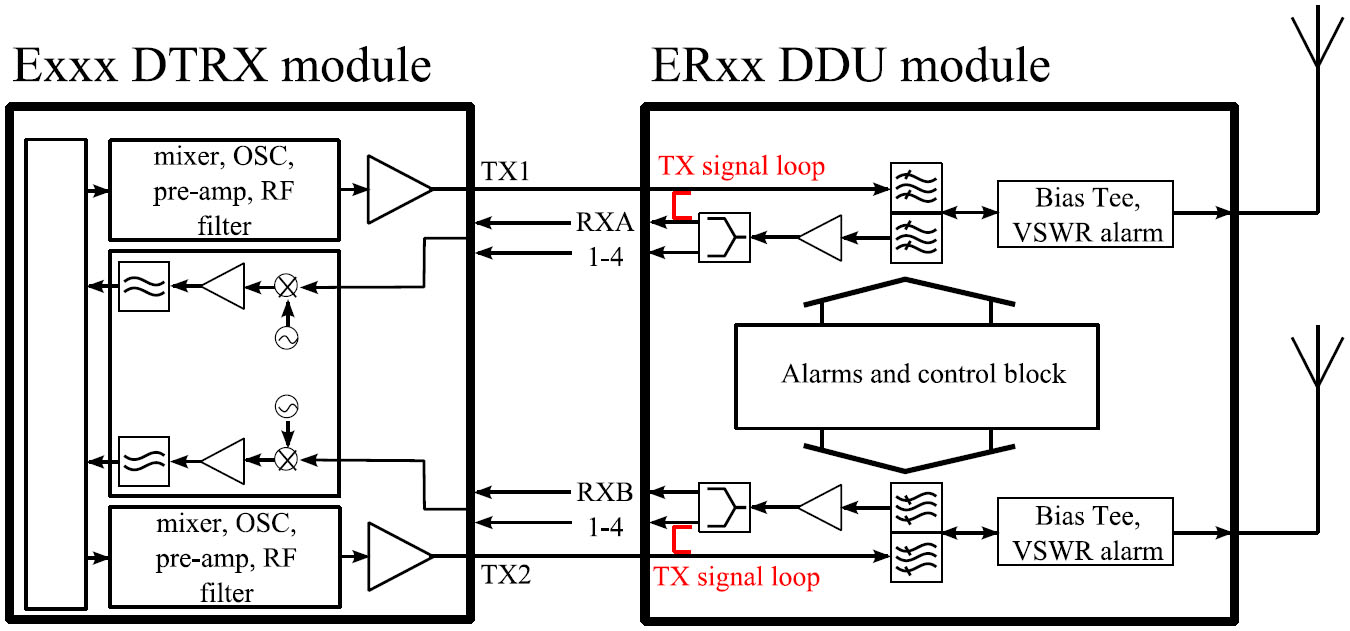
\includegraphics[width=\textwidth]{img/bs.jpg}
	\caption{Receiver under study.}
	\label{f:bs}
	\end{center}
	\vspace*{-12pt}
\end{figure}


\newpage
\section{Measurement steps}

In this section, used measurement configurations are presented for each measurement 
task. Measurements in question may be divided into two distinct categories: power 
measurements with a spectrum analyzer (SA) and two-port transmission measurements ($S_{21}$)
with a vector network analyzer (VNA). There were no significant differences between 
the planned setups and those used in the actual measurements. The following measuremeent 
specific subsections will elaborate.


\subsection{1~dB compression point}

To measure 1~dB compression point of a device, one needs a (manually) sweepable signal source 
and power detector. These may come separately or be incorporated in a single device. 
In both cases, the DDU module is connected the in between the source and the detector.
We used both approaches, and made two measurements with equal power levels.

For separate signal generation and detection, we used \textit{Rohde \& Schwarz SML03} signal 
generator (SG) and \textit{HP 8596E} spectrum analyzer.The measurement setup is shown in Figures 
\ref{f:sg1} and \ref{f:sg2}. The setup employing \textit{Rohde \& Schwarz ZVL} VNA is shown in 
Figures \ref{f:vna1} and \ref{f:vna2}. All equipment came precalibrated. In both measurements, 
the A-half of the base station was used.

\begin{figure}[h!]
	\begin{center}
	\setlength{\unitlength}{1mm}
	\begin{picture}(142, 13)
		\linethickness{0.2mm}
		\put(0, 0.4){\framebox[34mm]{Signal generator}}
		\put(34, 1.4){\vector(1,0){20}}
		\put(54, 0.4){\framebox[28mm]{$\mathrm{ANT} \rightarrow \mathrm{RX}_1$}}
		\put(82, 1.4){\vector(1,0){20}}
		\put(102, 0.4){\framebox[40mm]{Sprectrum analyzer}}
		\put(68, 7){\makebox(0,0){DDU module}}
	\end{picture}
	\vspace*{\halfLine}
	\caption{Measurement setup used in the first measurement task.}
	\label{f:sg1}
	\end{center}
	\vspace*{-12pt}
\end{figure}

\begin{figure}[h!]
	\begin{center}
	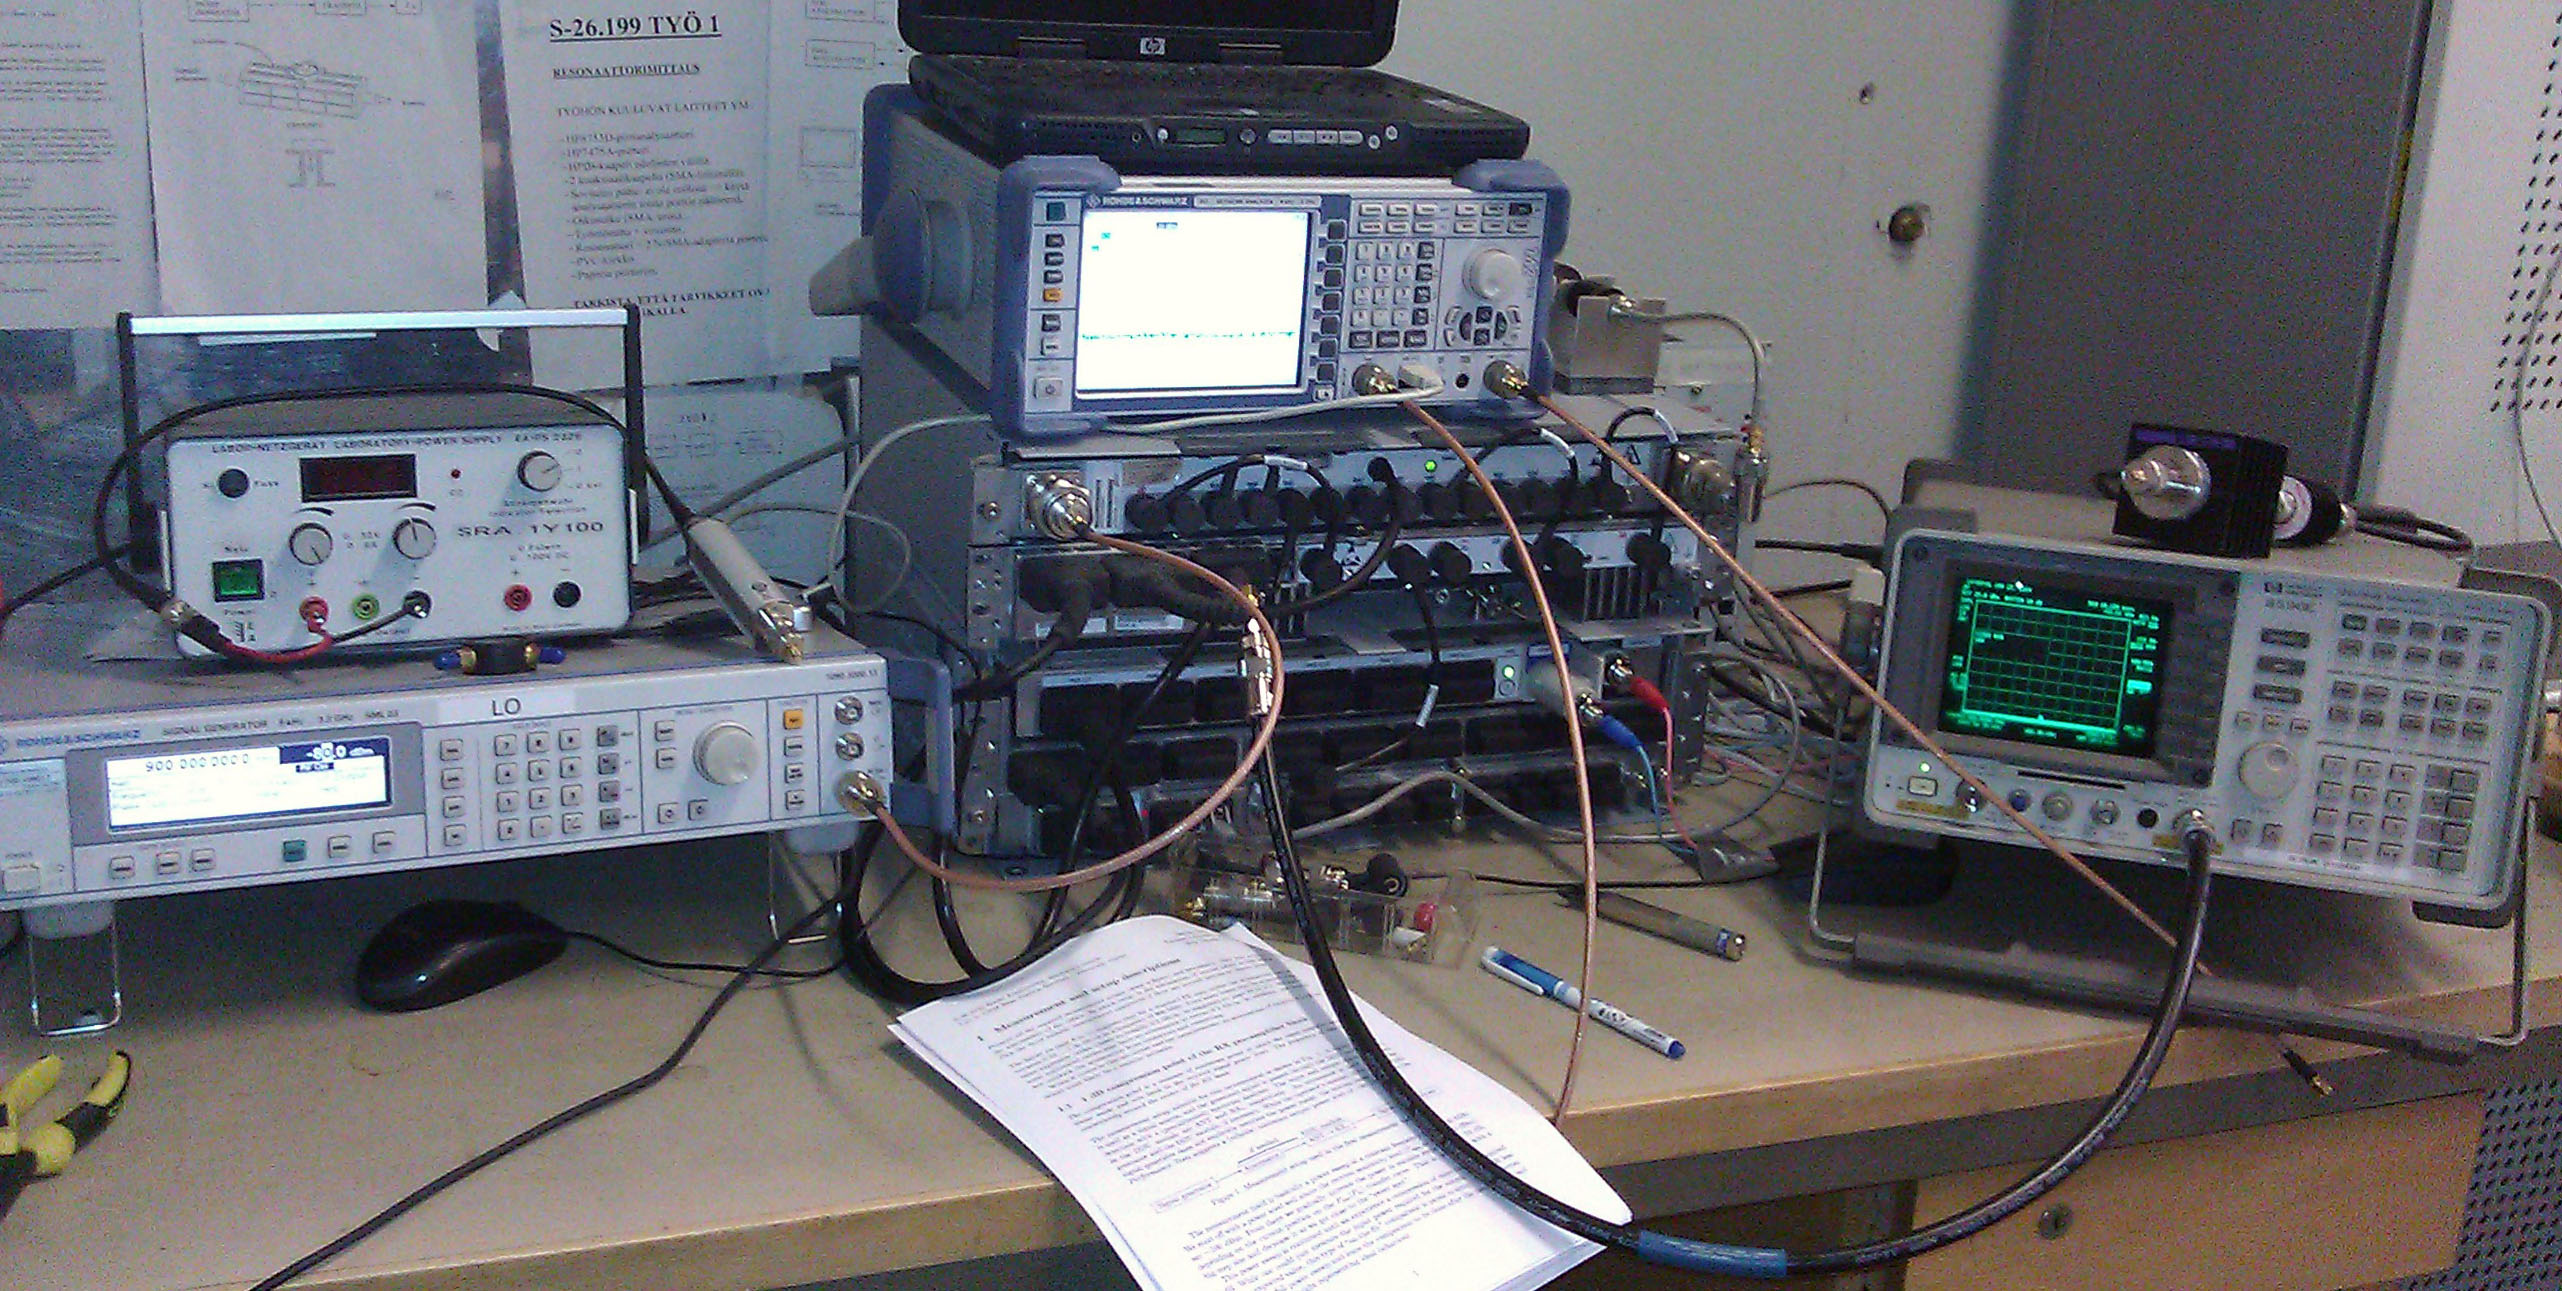
\includegraphics[width=0.75\textwidth]{img/sg-ddu-sa.jpg}
	\caption{Using a signal generator and spectrum analyzer to characterize the DDU module.}
	\label{f:sg2}
	\end{center}
	\vspace*{-12pt}
\end{figure}

\begin{figure}[h!]
	\begin{center}
	\setlength{\unitlength}{1mm}
	\begin{picture}(155, 10)
		\linethickness{0.2mm}
		\put(0, 0.4){\framebox[29mm]{VNA (Port 1)}}
		\put(29, 1.4){\vector(1,0){15}}
		\put(44, 0.4){\framebox[28mm]{$\mathrm{ANT} \rightarrow \mathrm{RX}_1$}}
		\put(72, 1.4){\vector(1,0){15}}
		\put(87, 0.4){\framebox[24mm]{Attenuator}}
		\put(111, 1.4){\vector(1,0){15}}
		\put(126, 0.4){\framebox[29mm]{VNA (Port 2)}}
		\put(58, 7){\makebox(0,0){DDU module}}
		\put(99, 7){\makebox(0,0){$L = 20$ dB}}
	\end{picture}
	\vspace*{\halfLine}
	\caption{VNA measurements connections}
	\label{f:vna1}
	\end{center}
	\vspace*{-12pt}
\end{figure}

\begin{figure}[h!]
	\begin{center}
	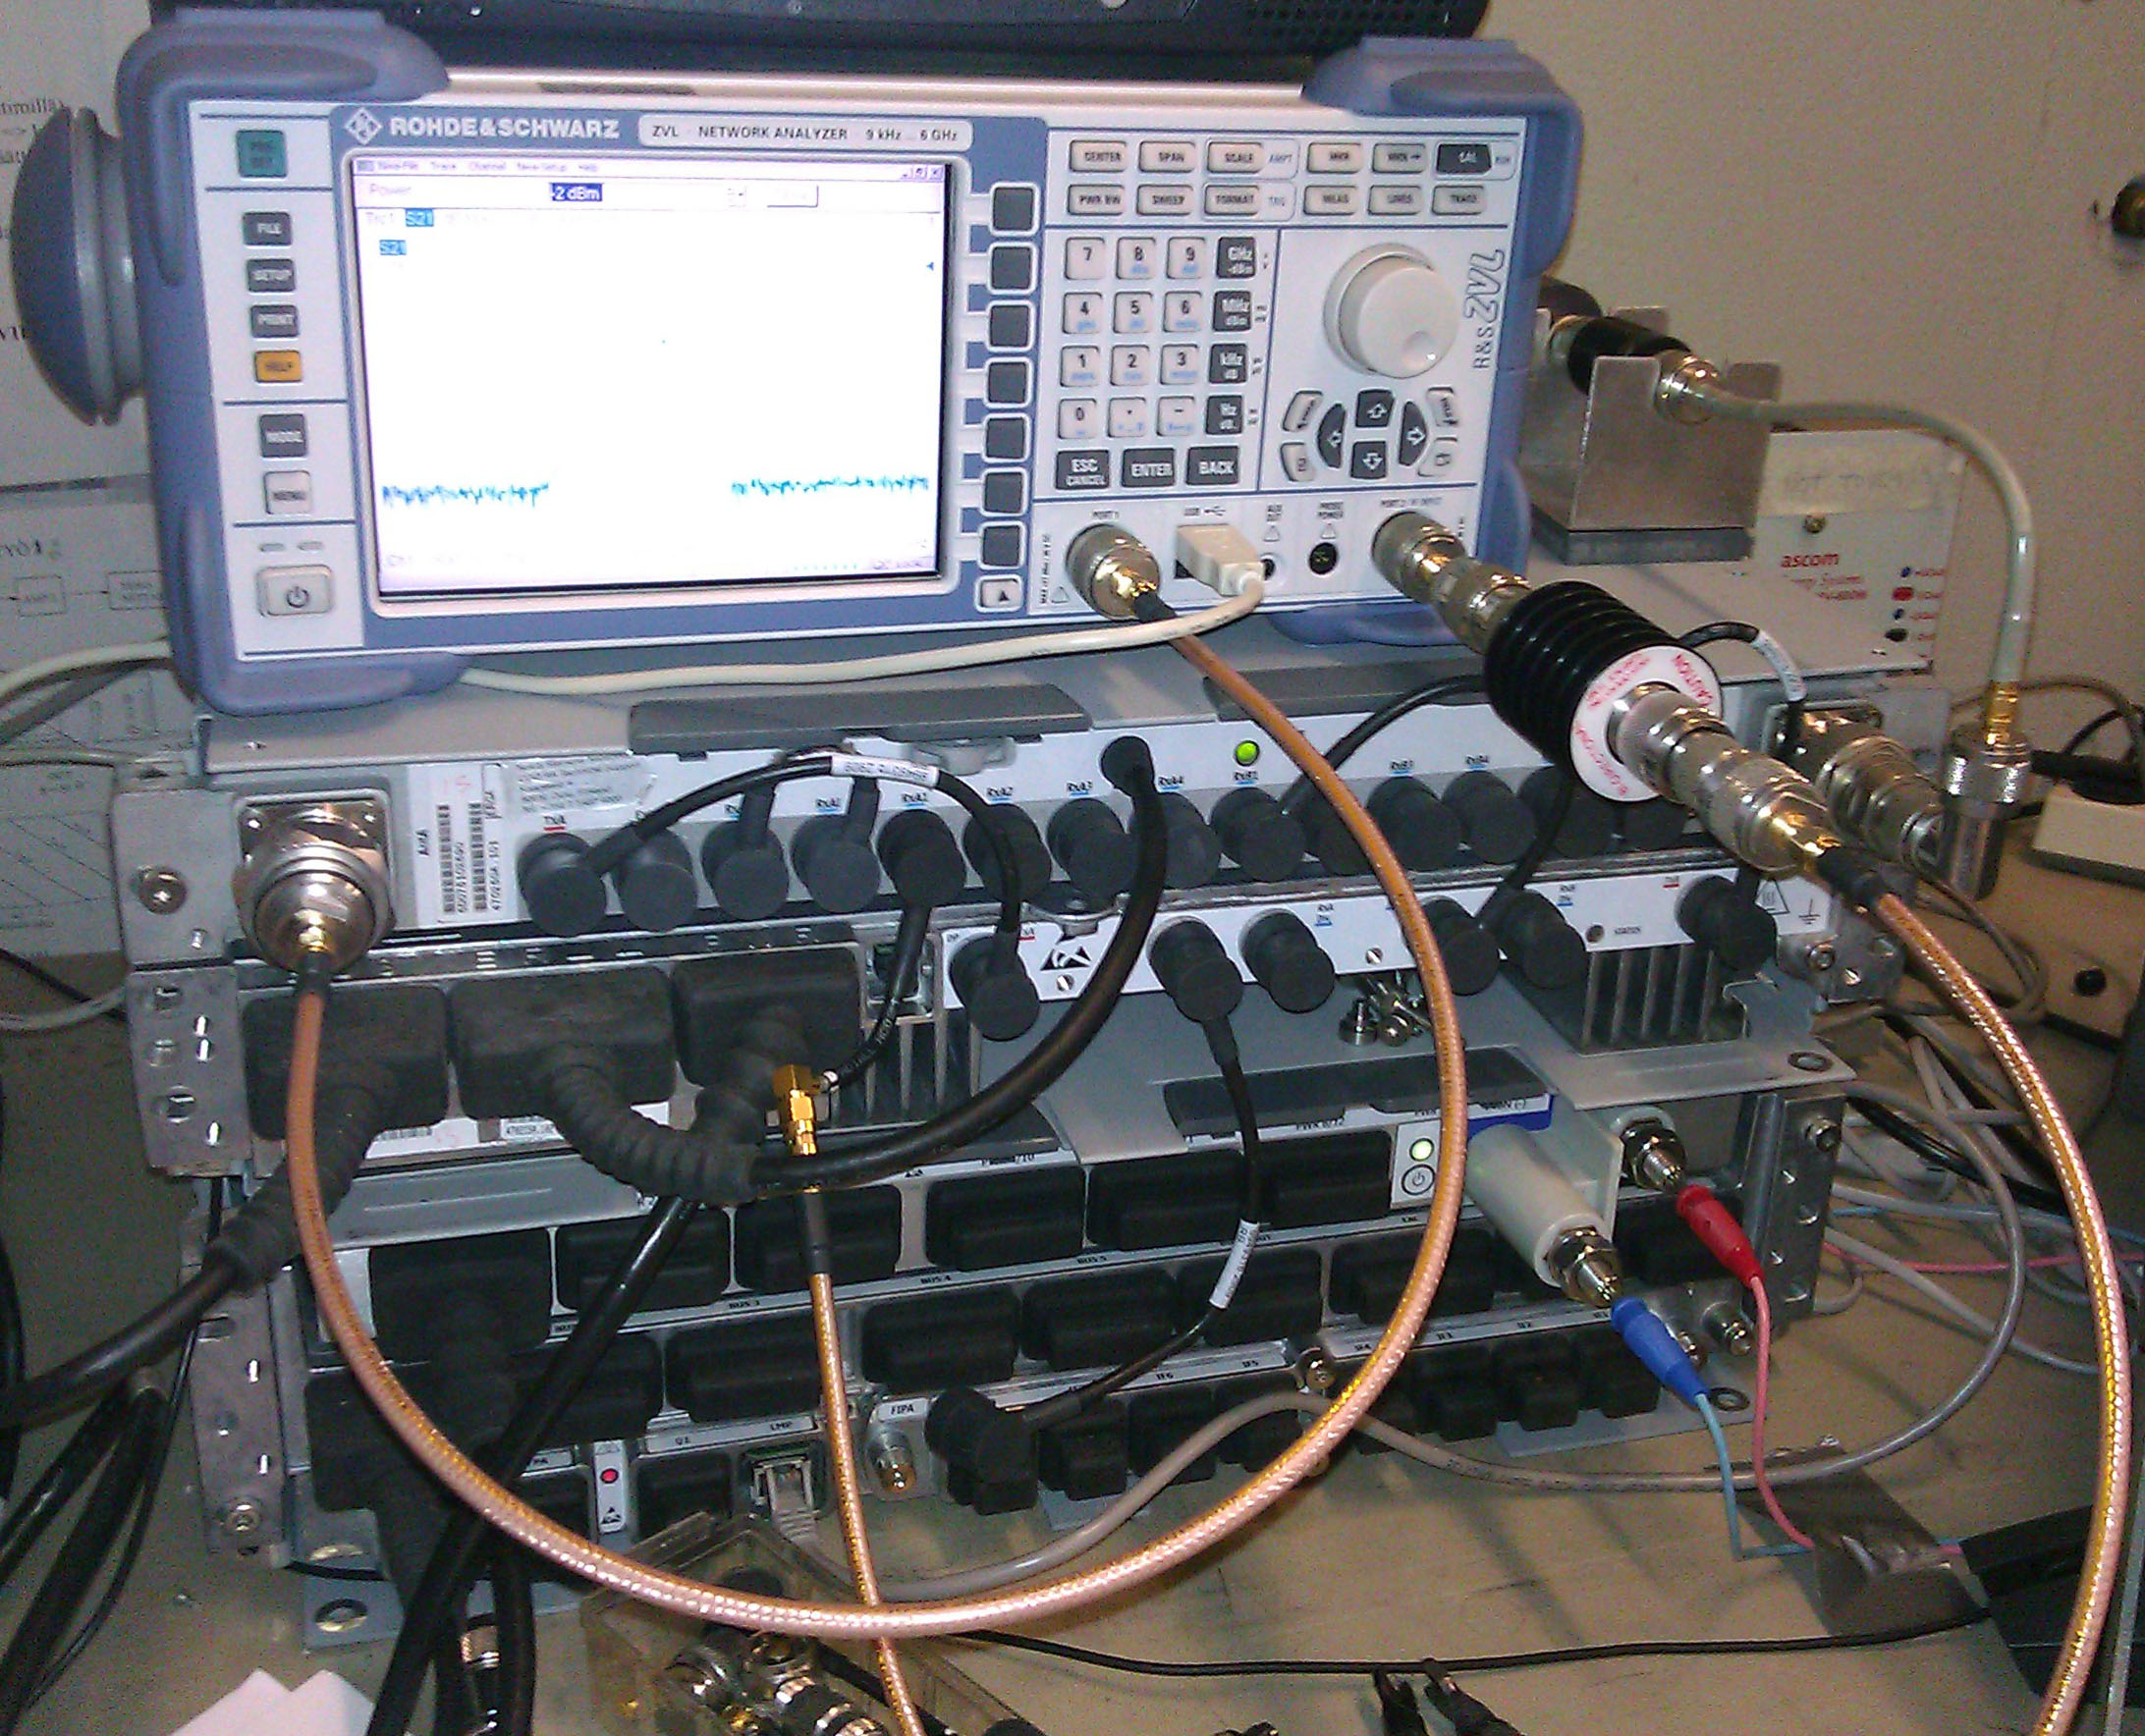
\includegraphics[width=0.75\textwidth]{img/vna-ddu-vna.jpg}
	\caption{Measuring the DDU module with the VNA.}
	\label{f:vna2}
	\end{center}
	\vspace*{-12pt}
\end{figure}

In essence, the measurement was a power sweep at a constant frequency of 
$f = 900$ MHz; mapping detected power or gain against used input power. 
This raw data was later postprocessed using Matlab.

We started with a source power of $-40$~dBm; a power level well below the 
1~dB compression point. The power was gradually used in steps of first 
10~dB, then 5~dB and finally 1~dB, until clear compression was observed. 
Compression may be seen in the lower than expected values of detected 
power (SG \& SA), or equivalently as lower gain (VNA).

Since we were measuring a GSM receiver, we used settings found in the GSM 
specification for the spectrum analyzer with the expeception of smaller 
averaging factor. They settings were as follows: an averaging factor of 100, 
zero span and 30~kHz video and resolution bandwidths. Input attenuation of the 
spectrum analyzer was increased from 10~dB all the way to 30~dB as we moved onto 
higher powers. 

The two cables and attenuators were measured separately using a VNA. For the VNA, 
the measurement settings throughout this lab were as follows: 1601 points over 
a frequency range of $800 \ldots 1000$~MHz, a measurement bandwidth of 10~kHz 
and averaging over 200 samples with a transmit power of $-20$~dBm.

For more accurate and/or reliable SA measurements, even a larger attenuation factor 
could have been used to avoid the small, yet possible, compression in the SA. One 
chould have also not trusted the quality of the SG as much than we did. The whole 
power sweep should have also been recorded without the DDU-module in between.
Also, there was some oversigth in making the connections as can be seen in 
Fig.~\ref{f:vna2}. As its only an attenuator in a transmission measurement, 
there is most likely no great an impact on the results as such. Nevertheless, 
it begs to question connector repeatability.


\subsection{Frequency response}

The frequency response was already measured in the first labs using a VNA. Thus 
we didn't need to measure the gain in these labs, as we used the results from 
the first labs. While the measurement procedure was given in the final report of 
the first labs, it is repeated here for completeness.

The measurement was carried out using a \textit{Rohde \& Schwarz ZVL} VNA, 
calibrated by the assistant prior to our arrival. The calibration settings were 
as follows: full two-port calibration with 1577 points within the $850 \ldots 1000$~MHz 
band, $-20$ dBm reference power, and an averaging factor of 100. The reference 
plane was located at the non-VNA end of the used cables.

The actual measurement included connecting the VNA to the B-half of the DDU module in 
order to obtain the values of $|S_{12}|$ over a set frequency range. In terms of physical 
connections, this would mean the following: VNA (Port~2) $\rightarrow$ DDU module 
(in: $\mathrm{ANT}_\mathrm{B}$, out: $\mathrm{RX}_\mathrm{B1}$) $\rightarrow$ VNA (Port~1). 
The raw data was stored onto a USB-memory as \texttt{*.s1p} files for post processing 
using Matlab.

The theoretical noise bandwidth $B_\mathrm{n}$ for a device may be found as using the 
following formula
\begin{equation}\label{e:Bn}
B_\mathrm{n} = \frac{1}{G_\mathrm{T,\;max}} \int_0^\infty G_\mathrm{T}(f) \, df,
\end{equation}
where $G_\mathrm{T}(f)$ is the transducer gain at frequency $f$. In practice, one may 
only approximate this using numerical integration over the finite measurement bandwidth. Such 
approximation is bound to yield slightly optimistic values. Another possibility is to 
approximate the noise bandwidth as the 3~dB bandwidth, and applying a compensation factor 
based on the transition bands. Results obtained using both methods are shown and compared 
later in the text.


\subsection{Noise temperature}

In the noise measurement task, we used the $Y$-coefficient method. The setup is shown 
in Figures \ref{f:nd1} and \ref{f:nd2}. A DC-voltage source is connected to a noise 
diode which is in turn connected by an SMA-cable to the $\mathrm{ANT}_\mathrm{A}$-input 
in the pre-amplifier block (A-half). It would have been better to use desired direct 
connection, but that was not possible due to missing adapters.

The signal is led then from the RX$_\mathrm{A1}$ output to the spectrum analyzer. We 
made another measurement where an amplifier was placed in between, as the noise power 
from the cold noise source might've been masked by the SA noise. The parameters of 
the amplifier, made by Minicircuits, were as follows: $B = 15 \ldots 3000$~MHz, 
$G = 19$~dB, $T = 463$~K, $F = 4.1$~dB and $V_\mathrm{CC} = +15$~V.

\begin{figure}[h!]
	\begin{center}
	\setlength{\unitlength}{1mm}
	\begin{picture}(163, 13)
		\linethickness{0.2mm}
		\put(0, 0.4){\framebox[10mm]{$V_\mathrm{DC}$}}
		\put(10, 1.4){\vector(1,0){12}}
		\put(22, 0){\framebox[25mm]{Noise diode}}
		\put(47, 1.4){\vector(1,0){12}}
		\put(59, 0.4){\framebox[28mm]{$\mathrm{ANT} \rightarrow \mathrm{RX}_1$}}
		\put(87, 1.4){\vector(1,0){12}}
		\put(99, 0.4){\framebox[12mm]{LNA}}
		\put(111, 1.4){\vector(1,0){12}}
		\put(123, 0.4){\framebox[40mm]{Sprectrum analyzer}}
		\put(5, 7){\makebox(0,0){0/28 V}}
		\put(73, 7){\makebox(0,0){DDU module}}
		\put(111, 8){\makebox(0,0){$\overbrace{\hspace{23mm}}^\textrm{with and without}$}}
	\end{picture}
	\vspace*{\halfLine}
	\caption{Noise temperature measurement setup}
	\label{f:nd1}
	\end{center}
	\vspace*{-12pt}
\end{figure}

\begin{figure}[h!]
	\begin{center}
	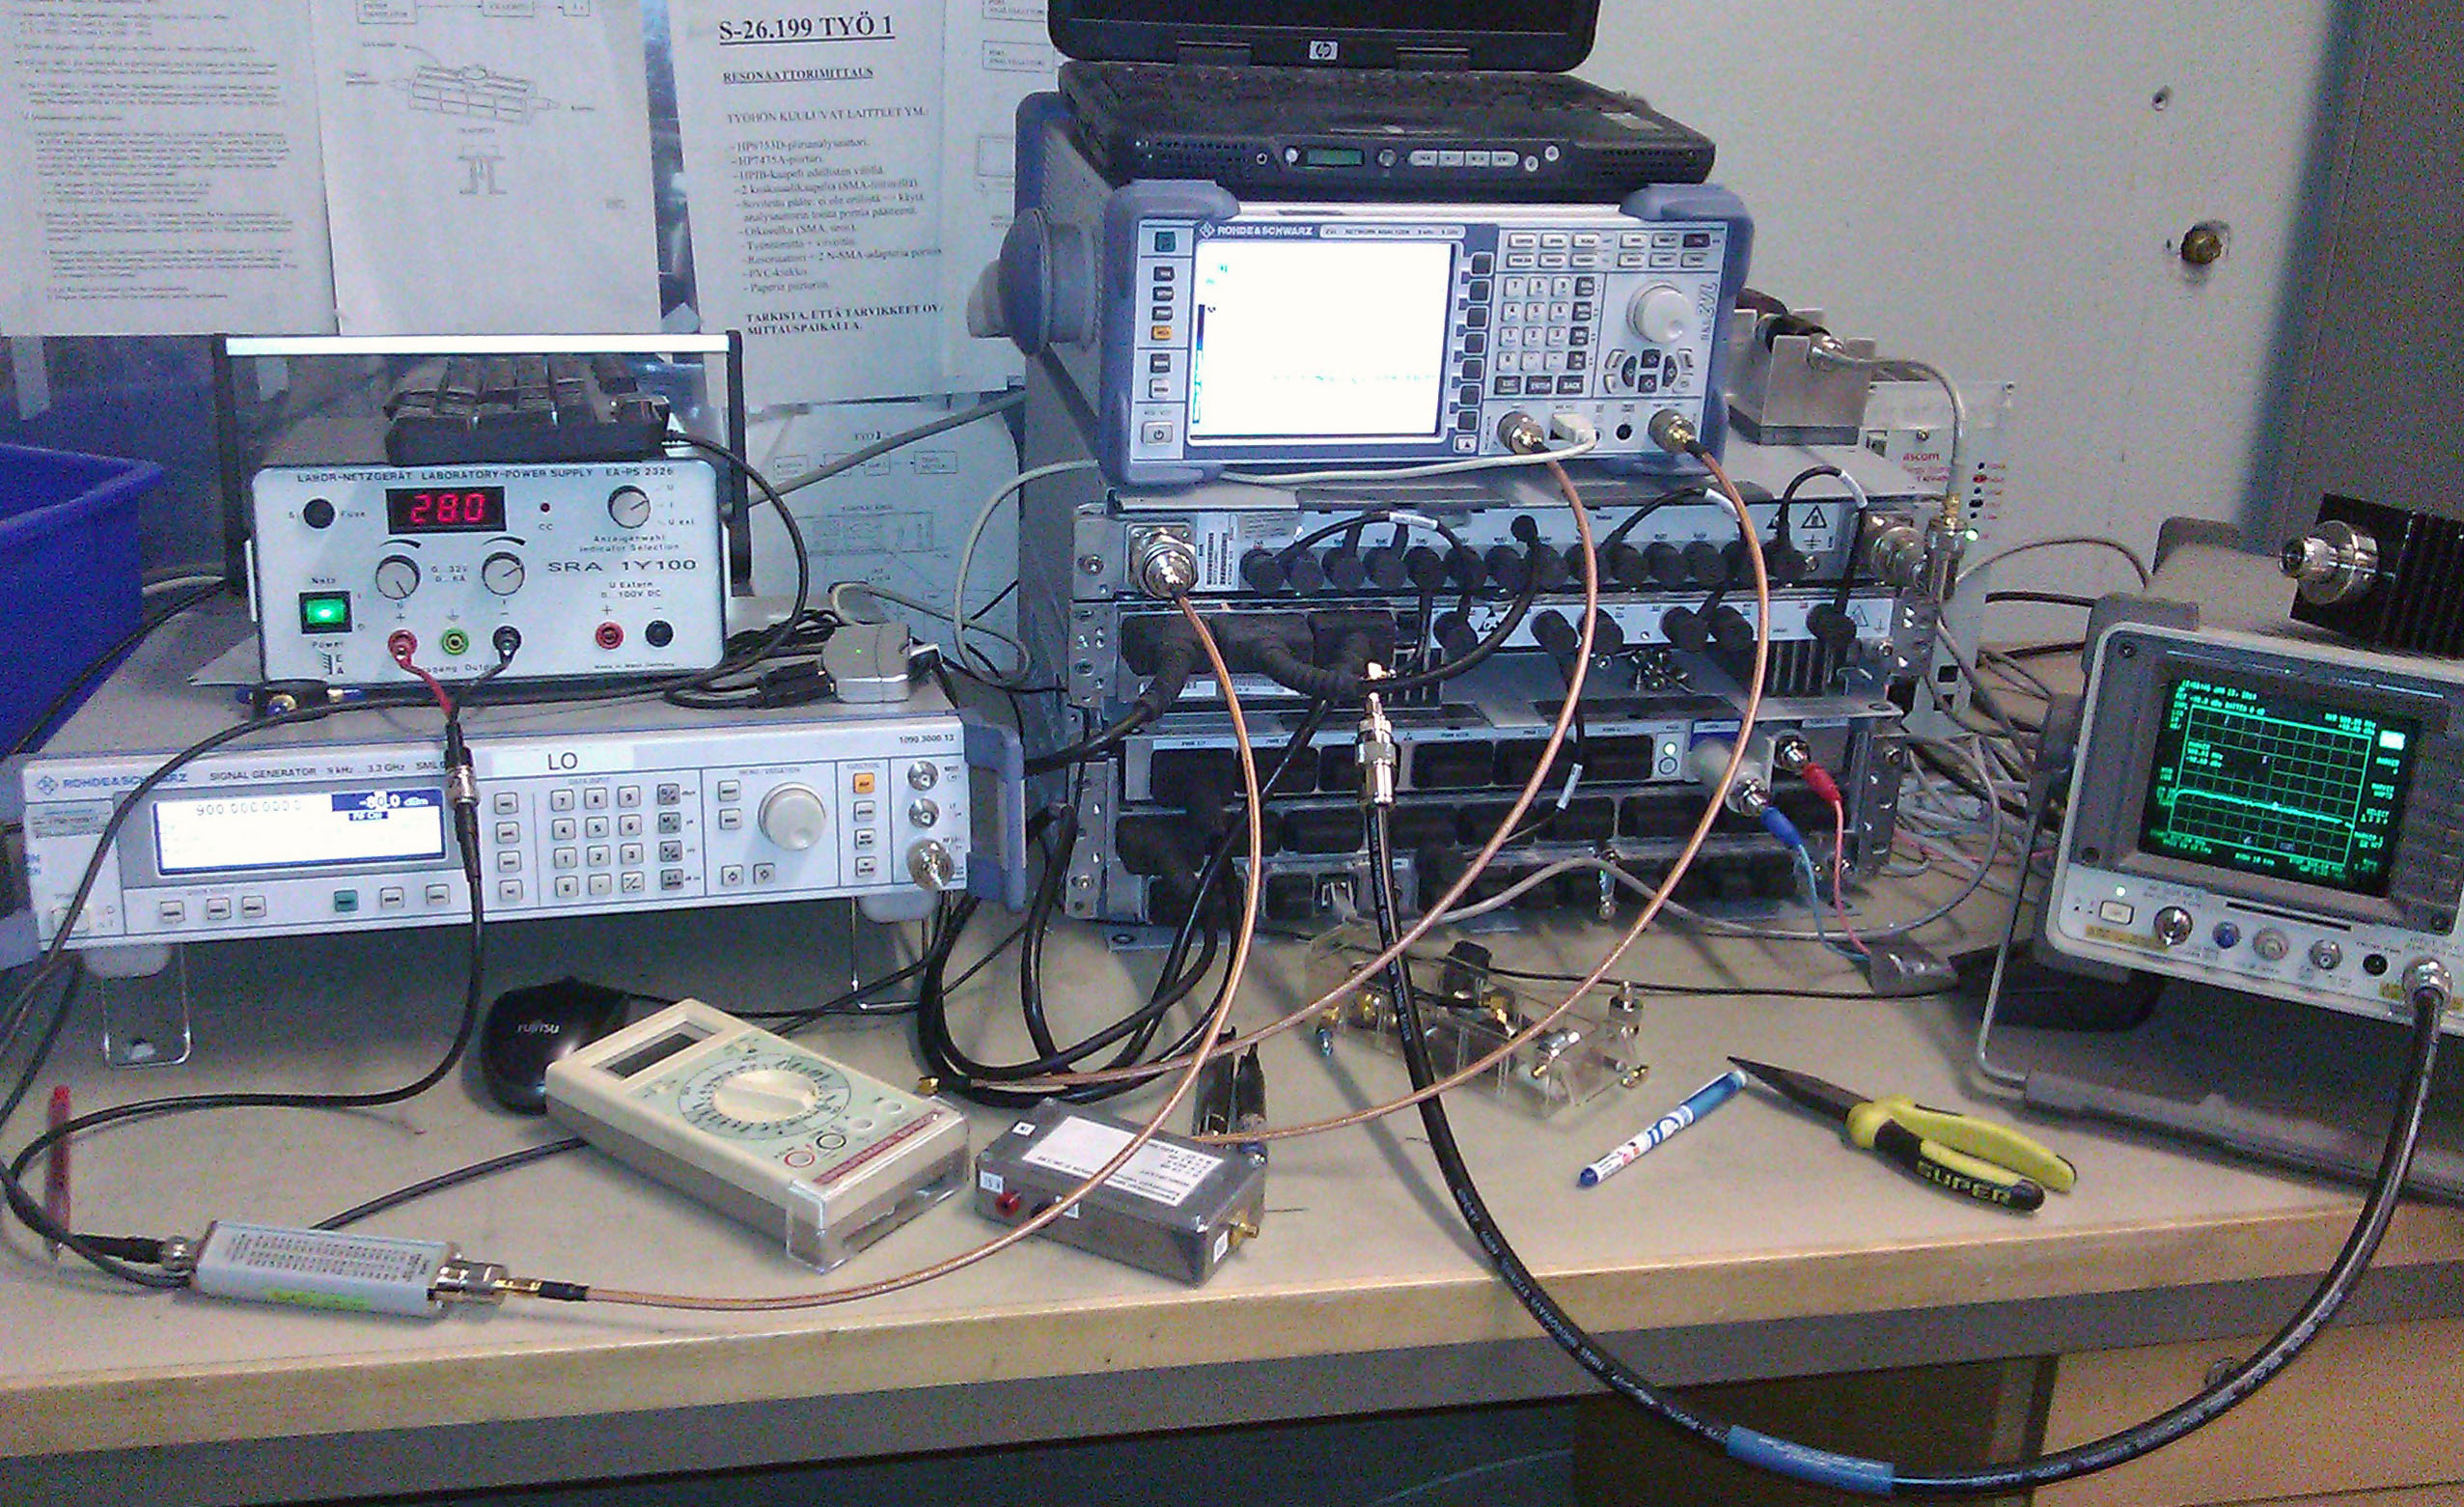
\includegraphics[width=0.75\textwidth]{img/nd-ddu-sa.jpg}
	\caption{Noise temperature measurement setup without the additional amplifier.}
	\label{f:nd2}
	\end{center}
	\vspace*{-12pt}
\end{figure}

The measurements themselves were carried out measuring two power levels required in the 
Y-pa\-ram\-e\-ter; when the DC-voltage is off/shorted (``cold'') and on (``hot''). We 
used \textit{HP 346B} noise diode ($\textit{ENR} = 21.48$~dB when $f = 1.00$~GHz) with 
a control voltage of 28~V$_\mathrm{DC}$ taken from a laboratory-grade voltage source.

As for the SA settings, the settings we as follows: 0~dB input attenuation, zero span, 
10~kHz resolution and video bandwidths and an averaging over 100 sweeps. For more accurate 
results, more time should have spent on this measurement. This would have allowed us to use 
smaller bandwidths and larger averaging factor.

The noise temperature, or equivalently noise factor/figure, may be found using the following
formulae. $Y$-coefficient is given as
\begin{equation}\label{e:Y}
Y = \frac{P_\mathrm{H}}{P_\mathrm{C}} 
	= \frac{T_\mathrm{H} + T_\mathrm{e}}{T_\mathrm{C} + T_\mathrm{e}}
	\quad\Rightarrow\quad
	T_\mathrm{e} = \frac{T_\mathrm{H} + YT_\mathrm{C}}{Y - 1},
\end{equation}
where $P_\mathrm{H/C}$ is the measured power for hot and cold loads at equivalent noise 
temperatures $T_\mathrm{H/C}$, and $T_\mathrm{e}$ is the noise temperature of the measured 
device. $T_\mathrm{C} = 295$~K is the physical temperature of the noise diode, and 
$T_\mathrm{H}$ may be solved from the definition of $\textit{ENR}$:
\begin{equation}
\mathit{ENR} = 10 \lg \left( \frac{T_\mathrm{H}}{T_\mathrm{C}} - 1 \right) 
	\quad\Rightarrow\quad
	T_\mathrm{H} = T_\mathrm{C} \left( 10^\frac{\mathit{ENR}}{10} + 1 \right).
\end{equation}
Obtained noise temperature $T_\mathrm{e}$ may be converted to noise factor $F$ or figure 
$F_\mathrm{dB}$ using the following relationship:
\begin{equation}
F_\mathrm{dB} = 10 \lg \left( F \right) \mathrm{\;dB} =  10 \lg \left( 1 + \frac{T_\mathrm{e}}{T_0} \right) \mathrm{\;dB}.
\end{equation}

One should notice that the $T_\mathrm{e}$ given by Eq.~\ref{e:Y} is actually the noise 
temperature of the whole chain. This chain is a cascaded system, consisting of a SMA-cable, 
the DDU module, the optional amplifier, another SMA-cable and the spectrum analyzer, in 
this order. The contribution of the DDU module may be determined by reverse calculating 
Friis' noise equation:
\begin{equation}
	F_\mathrm{total} = F_1 + \frac{F_2 - 1}{G_1} + \frac{F_3 - 1}{G_1 G_2} + \cdots
	\quad\Leftrightarrow\quad
	T_\mathrm{total} = T_1 + \frac{T_2}{G_1} + \frac{T_3}{G_1 G_2} + \cdots,
\end{equation}
where $G_i$ is the available power gain of the $i$th stage. Similar indexing is also used 
for both of the noise quantities $F$ and $T$. This simplified formula assumes equal noise 
bandwidths between the stages.

The parameters required by the formula may be obtained through calculation, or are provided 
by the manufacturer. For example the noise contribution of the cables can be obtained from 
their attenuation $L$ and physical temperature $T_\mathrm{phys}$ through formula 
$F = (L - 1) T_\mathrm{phys}$. The amplifier specifications were given already in the text.
For the spectrum analyzer, $F = ?$~dB.


\subsection{Sensitivity}

In the sensitivity measurement, we're measured the minimum input power at the ANT$_\mathrm{A}$-input 
that results in a reliably detectable signal above the noise floor in the ouput of the DDU module. 
In GSM-systems, a signal with $\mathit{SNR} > 10$~dB is detected with an acceptable $\mathit{BER}$. 
For this, a measurement setup identical to the one used in the first task may be used. The setup 
used there is shown in Figures \ref{f:sg1} and \ref{f:sg2}. An attenuator may be used between 
the signal generator and the DDU module.

\begin{figure}[h!]
	\begin{center}
	\setlength{\unitlength}{1mm}
	\begin{picture}(142, 13)
		\linethickness{0.2mm}
		\put(0, 0.4){\framebox[34mm]{Signal generator}}
		\put(34, 1.4){\vector(1,0){20}}
		\put(54, 0.4){\framebox[28mm]{$\mathrm{ANT} \rightarrow \mathrm{RX}_1$}}
		\put(82, 1.4){\vector(1,0){20}}
		\put(102, 0.4){\framebox[40mm]{Sprectrum analyzer}}
		\put(68, 7){\makebox(0,0){DDU module}}
	\end{picture}
	\vspace*{\halfLine}
	\caption{Measurement setup used in the sensitivity measurement.}
	\label{f:m4}
	\end{center}
	\vspace*{-12pt}
\end{figure}

The first step was to measure the noise floor at 900~MHz without any signal 
we're hoping to detect. That is, the RF power was switched off at the generator. 
Then we turned on an input signal that's some dBs below the reported sensitivity 
level of $-112.5$~dBm. We gradually increased the power until the signal-to-noise 
ratio was no less than the 10~dB required by the standard. The corresponding power 
level was recorded.

One could have also measure the power required to beat the noise just barely, and 
add the SNR later on. This approach is, however, less accurate and more painful. It 
also assumes $P_\mathrm{out}(P_\mathrm{in})$ relationship to be ideal in the range.

Since it's a GSM system, we use the measurement settings as they are defined in 
the standard with the exception of averaging. The standard 500-sweep averaging was 
used in when measuring the noise floow, but 100 was used when RF power was enabled. 
The final settings were as follows: an averaging factor of 500/100, zero span and 
30~kHz video and resolution bandwidths. The input attenuator was disabled in the 
SA settings.


\newpage
\section{Results}

TODO: Huy and Sampo (general results and intro to more specific results)


\subsection{1~dB compression point}

TODO: Huy and Sampo

\begin{figure}
\centering
\subcaptionbox{$P_\mathrm{out}(P_\mathrm{in})$ using SG \& SA}{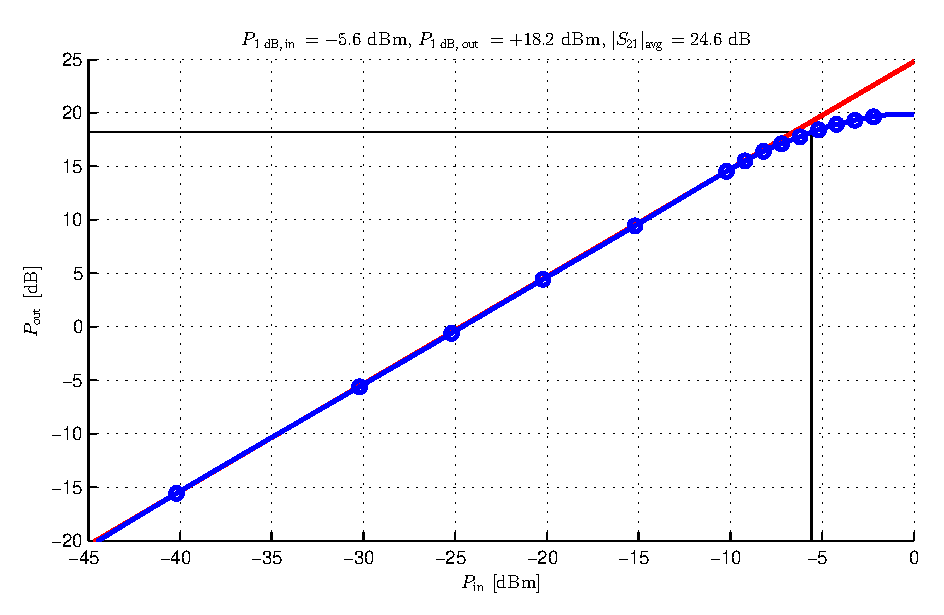
\epsfig{file=img/PoutPin1.eps, width=0.45\textwidth}}
\subcaptionbox{$P_\mathrm{out}(P_\mathrm{in})$ using VNA}{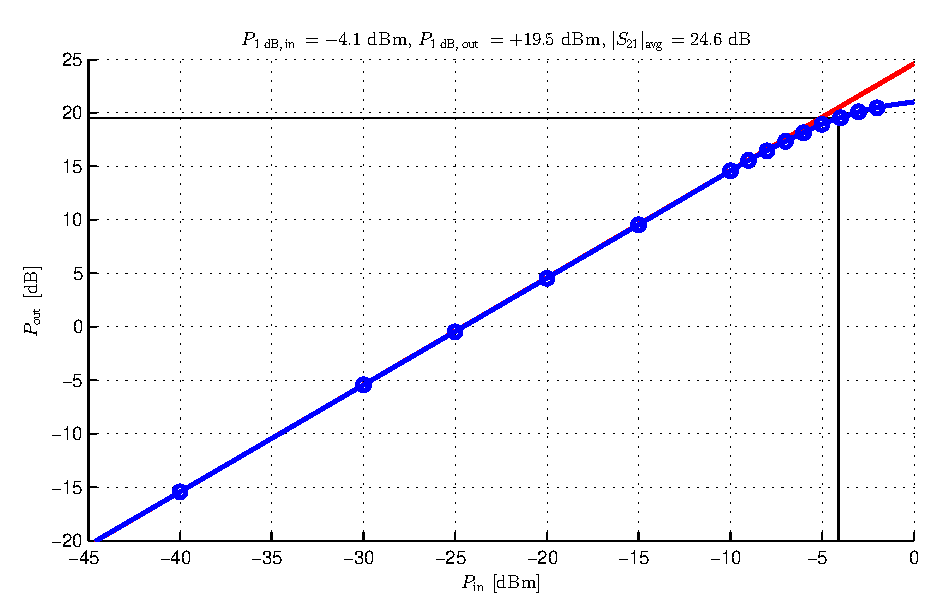
\epsfig{file=img/PoutPin2.eps, width=0.45\textwidth}}
\subcaptionbox{$G(P_\mathrm{in})$ using SG \& SA}{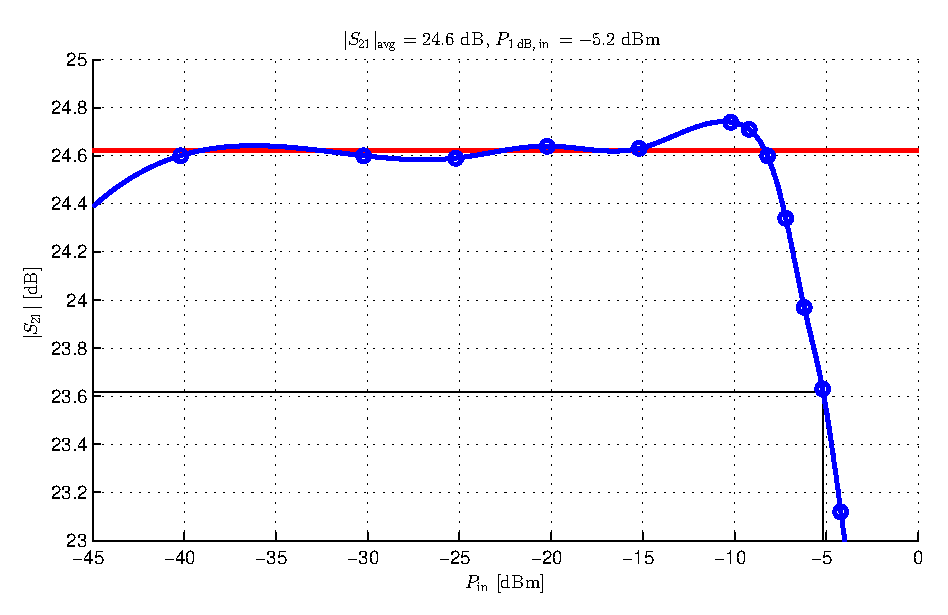
\epsfig{file=img/GPin1.eps, width=0.45\textwidth}}
\subcaptionbox{$G(P_\mathrm{in})$ using VNA}{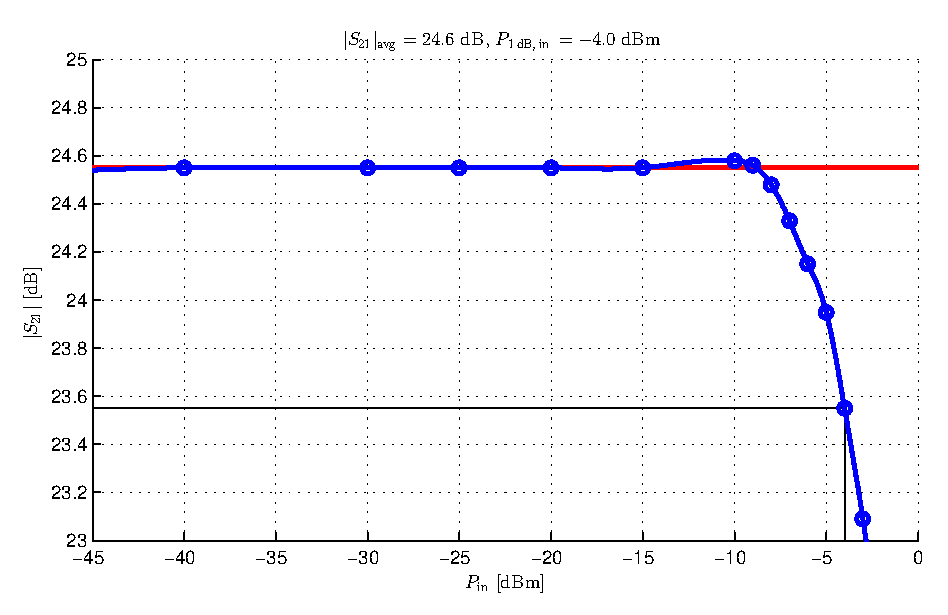
\epsfig{file=img/GPin2.eps, width=0.45\textwidth}}
\subcaptionbox{$G(P_\mathrm{out})$ using SG \& SA}{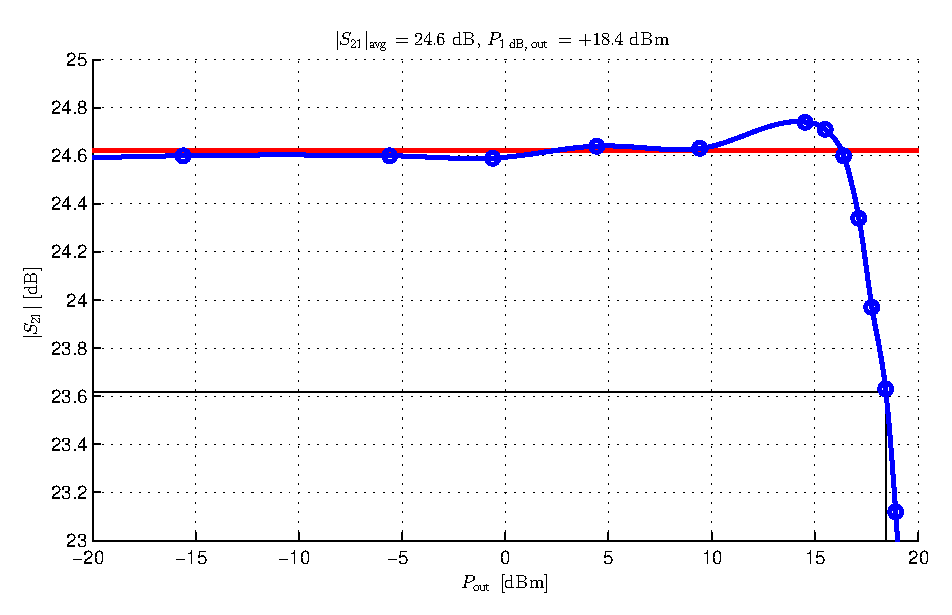
\epsfig{file=img/GPout1.eps, width=0.45\textwidth}}
\subcaptionbox{$G(P_\mathrm{out})$ using VNA}{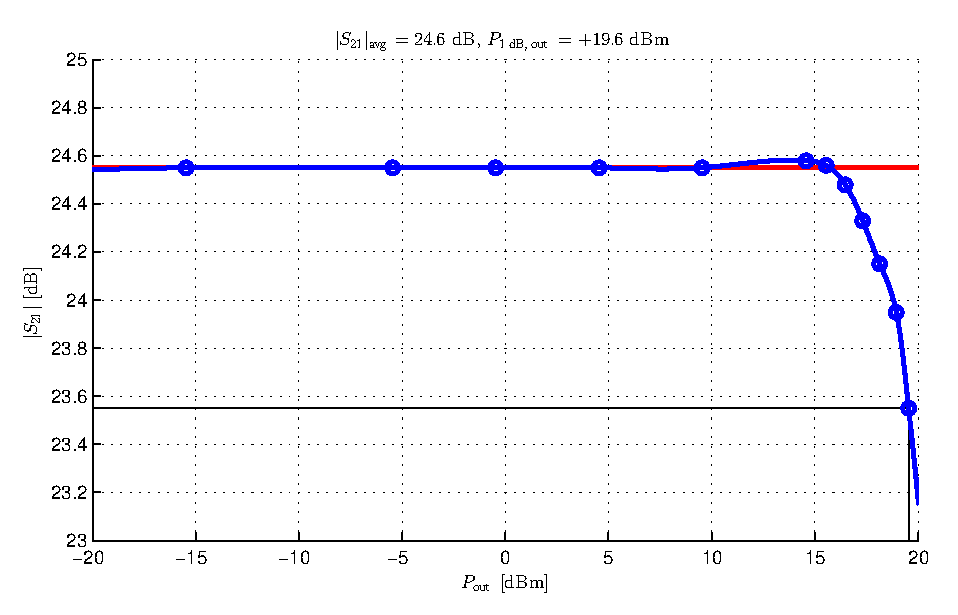
\epsfig{file=img/GPout2.eps, width=0.45\textwidth}}
\caption{Results from the 1~dB compression point measurements. Ideal behaviour is shown with red straights, 
	measuremets with blue markers and Matlab \texttt{'pchip'} interpolant in blue.}\label{f:1dB}
\end{figure}

\newpage
\subsection{Frequency response}

The $|S_{12}|$ response of the DDU module (B-half) within the $850 \ldots 1000$~MHz band 
is shown in the following figure (Fig.~\ref{f:s12}). In the figure, in addition to the 
actual response (in black), additional information is shown. GSM RX and TX band limits 
(in red), both 3~dB (in blue) and noise (in green) bandwidth of the pre-amp block are also 
visualized. Visualization of the noise bandwidth is somewhat questionable as it's a purely 
theoretical concept, but is nevertheless shown for scale. 

\begin{figure}[h!]
	\begin{center}
	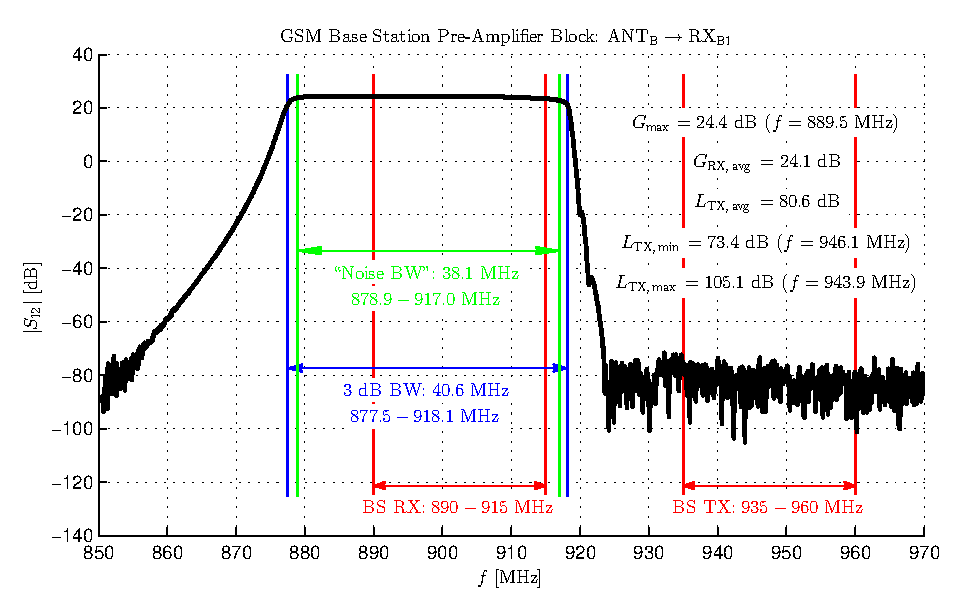
\epsfig{file=img/s12.eps, width=\textwidth}
	\caption{$S_{12}$ of the DDU module as was measured in the first labs.}
	\label{f:s12}
	\end{center}
	\vspace*{-12pt}
\end{figure}

The noise bandwidth shown, obtained from Eq.~\ref{e:Bn} is less than the actual band since 
we cannot use infinite frequency range. Frequency range of $850 \ldots 1000$~MHz with
$G_\mathrm{T,\;max} = |S_{12}|_\mathrm{max} = 24.4$~dB was used instead. The obtained 
value (38.1~MHz) is roughly 6~\% shy of the 3~dB bandwidth (40.6~MHz), as one might expect.
The 3~dB bandwidth may thus be used to avoid being overly optimistic.

In the graphical approximation method we need to investigate the effect of frequency 
roll-off speed. From Fig.~\ref{f:s12} the transition bands are approx. 30~MHz (3.4 \%) 
and 5~MHz (0.55 \%) for lower and upper bands, respectively. During this transition, 
the $S_12$ drops roughly 100~dB from $+20$~dB to $-80$~dB. This corresponds to a slope 
of $3.3$~dB/MHz (29~dB/\%) and $-20$~dB/MHz ($-180$~dB/\%), respectively. The effect of 
such steep slopes are neglectable, and thus the 3~dB bandwidth may be used as the noise 
bandwidth.


\subsection{Noise Temperature}

TODO: Huy and Sampo

\begin{table}[!h]
	\begin{center}
	\caption{Results from the noise measurement.}
	\label{t:noise}
	\renewcommand*{\arraystretch}{1.2}
	\begin{tabular}{cccccc}
	LNA? 			& $P_\mathrm{C}$ [dBm] 		& $P_\mathrm{H}$ [dBm]	& $T_\mathrm{total}$ [K] 	& $T_\mathrm{DDU}$ [K] 	& $F_\mathrm{DDU}$ [dB] \\
	\hline
	No				& $-107.3$					& $-90.8$				&  							&  						& \\
	Yes				& $-91.3$					& $-71.7$				&  							&  						&  	
	\end{tabular}
	\end{center}
	\vspace*{-12pt}
\end{table}


\subsection{Sensitivity}

TODO: Huy and Sampo

\begin{table}[!h]
	\begin{center}
	\caption{Results from the sensitivity measurement. The noise floor was measured to be at $-101.98$~dBm.}
	\label{t:sens}
	\renewcommand*{\arraystretch}{1.2}
	\begin{tabular}{cc}
	$\mathit{SNR}$ [dB] 			& $P_\mathrm{transmit}$ [dBm]  \\
	\hline
	7.5								& $-118.0$ 	\\
	10								& $-115.6$ 	\\
	12.5							& $-113.0$ 	
	\end{tabular}
	\end{center}
	\vspace*{-12pt}
\end{table}


\subsection{Dynamic range}

TODO: Huy and Sampo (refer to 1dB comp and sens.)


\newpage
\section{Error estimates}

TODO: Huy and Sampo (make additions, corrections, change the style to avoid excess 
repetition etc.)

In this section, error estimates for the two types of measurements are presented.
The values presented here are only rough estimates based on literature (with more 
or less general cases) and their soundness in this case is somewhat questionable. 
In this section, we do not take human errors (see previous section) into account. 
It is just stated that systematic errors arising from the cables and connections 
are possible in measurement all measurements. Thus they are valid only for 
``correct'' measurements, and are more of the ``provided for completeness'' 
nature. Probabilities are not given due to the nature/basis of the estimation.


\subsection{Spectrum analyzer}

Each of the components inside the spectrum analyzer contributes to the total uncertainty, 
depending for example on the signal frequencies, amplitudes, and measurement settings. 
The Agilent (former HP, manufacturer of the used SA) has made available a document that 
specifies the different error sources, giving also rough estimates for some spectrum 
analyzers. According to the document \cite{sa}, the error estimates vary broadly among 
different analyzer models, giving worst case uncertainties exceeding $\pm 6$ dB. On the 
other hand, the document gives also representative values of amplitude uncertainties, 
which in our case yields about $\pm 1$ dB.

The second error source for the spectrum analyzer is the power marker reading. In 
each of the tasks, the spectrum analyzer was set to average 500 measurement points, 
which should average out most of the random errors. However, reading the power marker 
in the screen, there was a noticeable fluctuation in the shown power value. Based on the 
experience obtained during the measurements, the power marker error is estimated to be 
approximately $\pm 0.5$ dB.

In conclusion, the error estimates that can be taken into account numerically are 
the manufacturers representative value of approx. $\pm 1$ dB, and the power marker 
fluctuation of roughly $\pm 0.5$ dB. These uncorrelated errors may be summed to 
achieve the total uncertainty of the SA measurements of approx. $\pm 1.5$ dB. 

There is also the question of calibrating the spectrum analyzer properly with 
the time interval defined by the manufacturer. Agilent suggests to have the spectrum 
analyzer calibrated thoroughly once in a year, and quick-calibrated if there are 
changes operating environment \cite{sa2}. If the spectrum analyzer used in the 
measurements is not calibrated correctly, it is possible that the measurements are 
not reliable. In this case, the calibration is the most important error source, and 
the device should be calibrated correctly before estimating any other errors.


\subsection{Vector network analyzer}

For the VNA, different error sources and ways to cope with them are listed in the 
lecture slides discussing VNA measurements. The different sources are noise, 
cabling/connector repeatability, directivity, isolation, mismatch and environment 
induced drift. 

Noise and cabling/connector repeatability are random errors, which can be averaged 
out. In our case, only the noise was averaged, since we did not touch the cabling. 
Systematic errors arising directivity, isolation, and mismatch in this task were
for the most part neglected with a calibration. Before conducting measurements, 
the VNA is always calibrated using a standard calibration module. The calibration 
moves the reference planes to the connectors of the test cables, and somewhat 
cancels the systematic errors from the connectors and cables used in a specific 
measurement. Finally, the environment induced drift is not relevant, since the 
measurement was done inside a short time interval.

Rohde \& Schwarz provides specifications that describe the measurement uncertainty 
of the VNA in question in different frequency bands. For transmission measurements 
in the frequency range of 50 MHz to 3 GHz, accuracy for signal powers of $-50 \ldots 0$ 
dB is better than $0.2$ dB ($0.3$ dB for powers of $-50 \ldots {-70}$ dB) with 0 dBm 
transmit power. \cite{vna} The reader should note that these ranges was exceeded 
from both ends during the measurements (the measurement power range was roughly 
$-100 \ldots {+4}$ dBm). 

In conclusion, two things are assumed. First, calibration is assumed to cancel the 
systematic errors arising from cables and connectors. Second, random errors are 
cancelled with averaging. The manufacturer provides error estimates for the device 
itself, giving an error estimate of under $0.3$ dB that is mostly applicable in 
our case. The topics discussed in the last paragraph of the last subsection apply 
here to some extent to here as well.


\subsection{Noise diode}

See lecture handout supplement.


\newpage
\section{Conclusions}

TODO: Huy and Sampo


\newpage
\section{Feedback}

TODO: Huy and Sampo (not all devices are listed in the instructions sheet, learning from feedback, sweeptime)


\newpage
\begin{thebibliography}{9}%\itemsep 7pt\parskip -5pt 

\bibitem{lab2} C.\ Icheln, S.\ Khanal, 
	\textit{GSM Receiver laboratory assignment instructions},
	S-26.3120 Laboratory course in Radio Engineering course material.
	
\bibitem{} C.\ Icheln (edited), 
	\textit{Lecture supplement handout},
	S-26.3120 Laboratory course in Radio Engineering course material.

\bibitem{sa} Agilent, Spectrum Analysis Basics, Application Note 150. 
	Available online at \url{http://cp.literature.agilent.com/litweb/pdf/5952-0292.pdf} 
	[Retrieved: Jan 2nd, 2014].
	
\bibitem{sa2} Agilent, 8590 Series Analyzers Calibration Guide.
	Available online at \url{http://cp.literature.agilent.com/litweb/pdf/08594-90106.pdf}
	[Retrieved: Jan 2nd, 2014].
	
\bibitem{vna} R\&S ZVL Vector Network Analyzer Specifications, 
	Version 06.00, Dec 2008. 
	Available online at \url{http://www.upc.edu/pct/documents_equipament/d_160_id-655-2.pdf} 
	[Retrieved: Jan 2nd, 2014].


%\bibitem{pozar} D.\ M.\ Pozar, 
%	\textit{Microwave Engineering}, 
%	J.\ Wiley \& Sons, 4th Edition, 2012. 
%	ISBN: 978-0-470-63155-3.
	
%\bibitem{gains} J.\ C.\ Logan, J.\ W.\ Rockway, 
%	``Dipole and Monopole Antenna Gain and Effective Area for Communication Formulas.''
%	Available online at \url{www.dtic.mil/cgi-bin/GetTRDoc?AD=ADA332891}
%	[Retrieved: November 25, 2013].

%\bibitem{parts} M.\ Steer, 
%	\textit{Microwave and RF Design -- A Systems Approach}, 
%	SciTech Publishing, 2010. 
%	ISBN: 978-1-891-12188-3.
	
%\bibitem{iet} R.\ J.\ Collier, A.\ D.\ Skinner (editors), 
%	\textit{Microwave Measurements}, 
%	The Institution of Engineering and Technology, 3rd Edition, 2007. 
%	ISBN: 978-0-86341-735-1.

\end{thebibliography}

\end{document}
